\documentclass[11pt,a4paper]{article}

\usepackage[margin=22mm]{geometry}
\usepackage{amsmath}
\usepackage{booktabs}
\usepackage{graphicx}
\usepackage[hidelinks]{hyperref}
\usepackage{microtype}
\usepackage[section]{placeins}
\usepackage{tabularx}
\usepackage{xcolor}

\graphicspath{{figures/}}
\setlength{\parindent}{0pt}
\setlength{\parskip}{0.55em}
\renewcommand{\arraystretch}{1.18}

\title{\textbf{Basilisk MPI CPU Benchmarks for Multiphase Flow}}
\author{Vatsal Sanjay\\
\small Computational Multiphase Physics (CoMPhy) Lab\\
\small Department of Physics, Durham University\\
\small \url{https://comphy-lab.org/}}
\date{September 2026}

\begin{document}
\maketitle

\begin{abstract}
Basilisk is an open-source framework for solving interfacial flows on
quadtree and octree meshes. Its pressure projection places a multigrid
Poisson solve inside every incompressible time step, making communication
across mesh levels a direct measure of the strong-scaling limit. This report
sets out a portable CPU benchmark suite built from two stock Basilisk kernels
and one representative two-phase calculation. Measurements on MareNostrum~5
and Snellius cover up to 16,384 MPI ranks for fixed-size kernel problems and
up to 1,024 ranks for the application cases. The kernel data support
small-to-medium system qualification and expose the onset of
communication-limited scaling. Tests above 100 fully populated 192-core nodes
remain a proposed campaign rather than a demonstrated result.
\end{abstract}

\section{What the benchmark measures}

An incompressible Basilisk calculation advances advection, viscosity and
interfacial forces before projecting the velocity field onto a divergence-free
space. The projection requires a multigrid Poisson solve. Restriction and
prolongation transfer information between mesh levels, while the domain
decomposition exchanges data between MPI ranks. At sufficiently large rank
counts, this communication ceases to be hidden by the work performed on each
rank. A fixed-size rank sweep therefore identifies both the useful
strong-scaling range and the point at which adding CPUs no longer reduces the
time to solution.

The proposed suite has three layers:
\begin{enumerate}
  \item stock Poisson and Laplacian kernels for reproducible machine-to-machine
        comparison;
  \item a verified two-phase migration problem that exercises the same solver
        stack with interface reconstruction and surface tension; and
  \item a workload series in which spatial resolution or the number of drops
        is increased, testing whether a larger application postpones
        strong-scaling saturation.
\end{enumerate}

The source cases, compact timing tables and plotting scripts are maintained at
\url{https://github.com/comphy-lab/hpc-basilisk-scaling}. The stock kernel
sources are retained without modification from the corresponding Basilisk
tests~\cite{basilisk-mpi-circle,basilisk-mpi-laplacian}.

\section{Kernel benchmark evidence}

The two-dimensional kernel uses a full quadtree at level $L=14$, corresponding
to $2^{28}$ cells. Figure~\ref{fig:2d-kernel} compares wall-clock and MPI time
on MareNostrum~5 and Snellius with the published Curie measurements. On
Snellius, the Poisson time continues to decrease through 8,192 ranks and is
unchanged within the resolution of this single-run dataset at 16,384 ranks.
The simultaneous rise in the communication fraction identifies the
large-rank regime as communication limited rather than compute limited.

\begin{figure}[htbp]
  \centering
  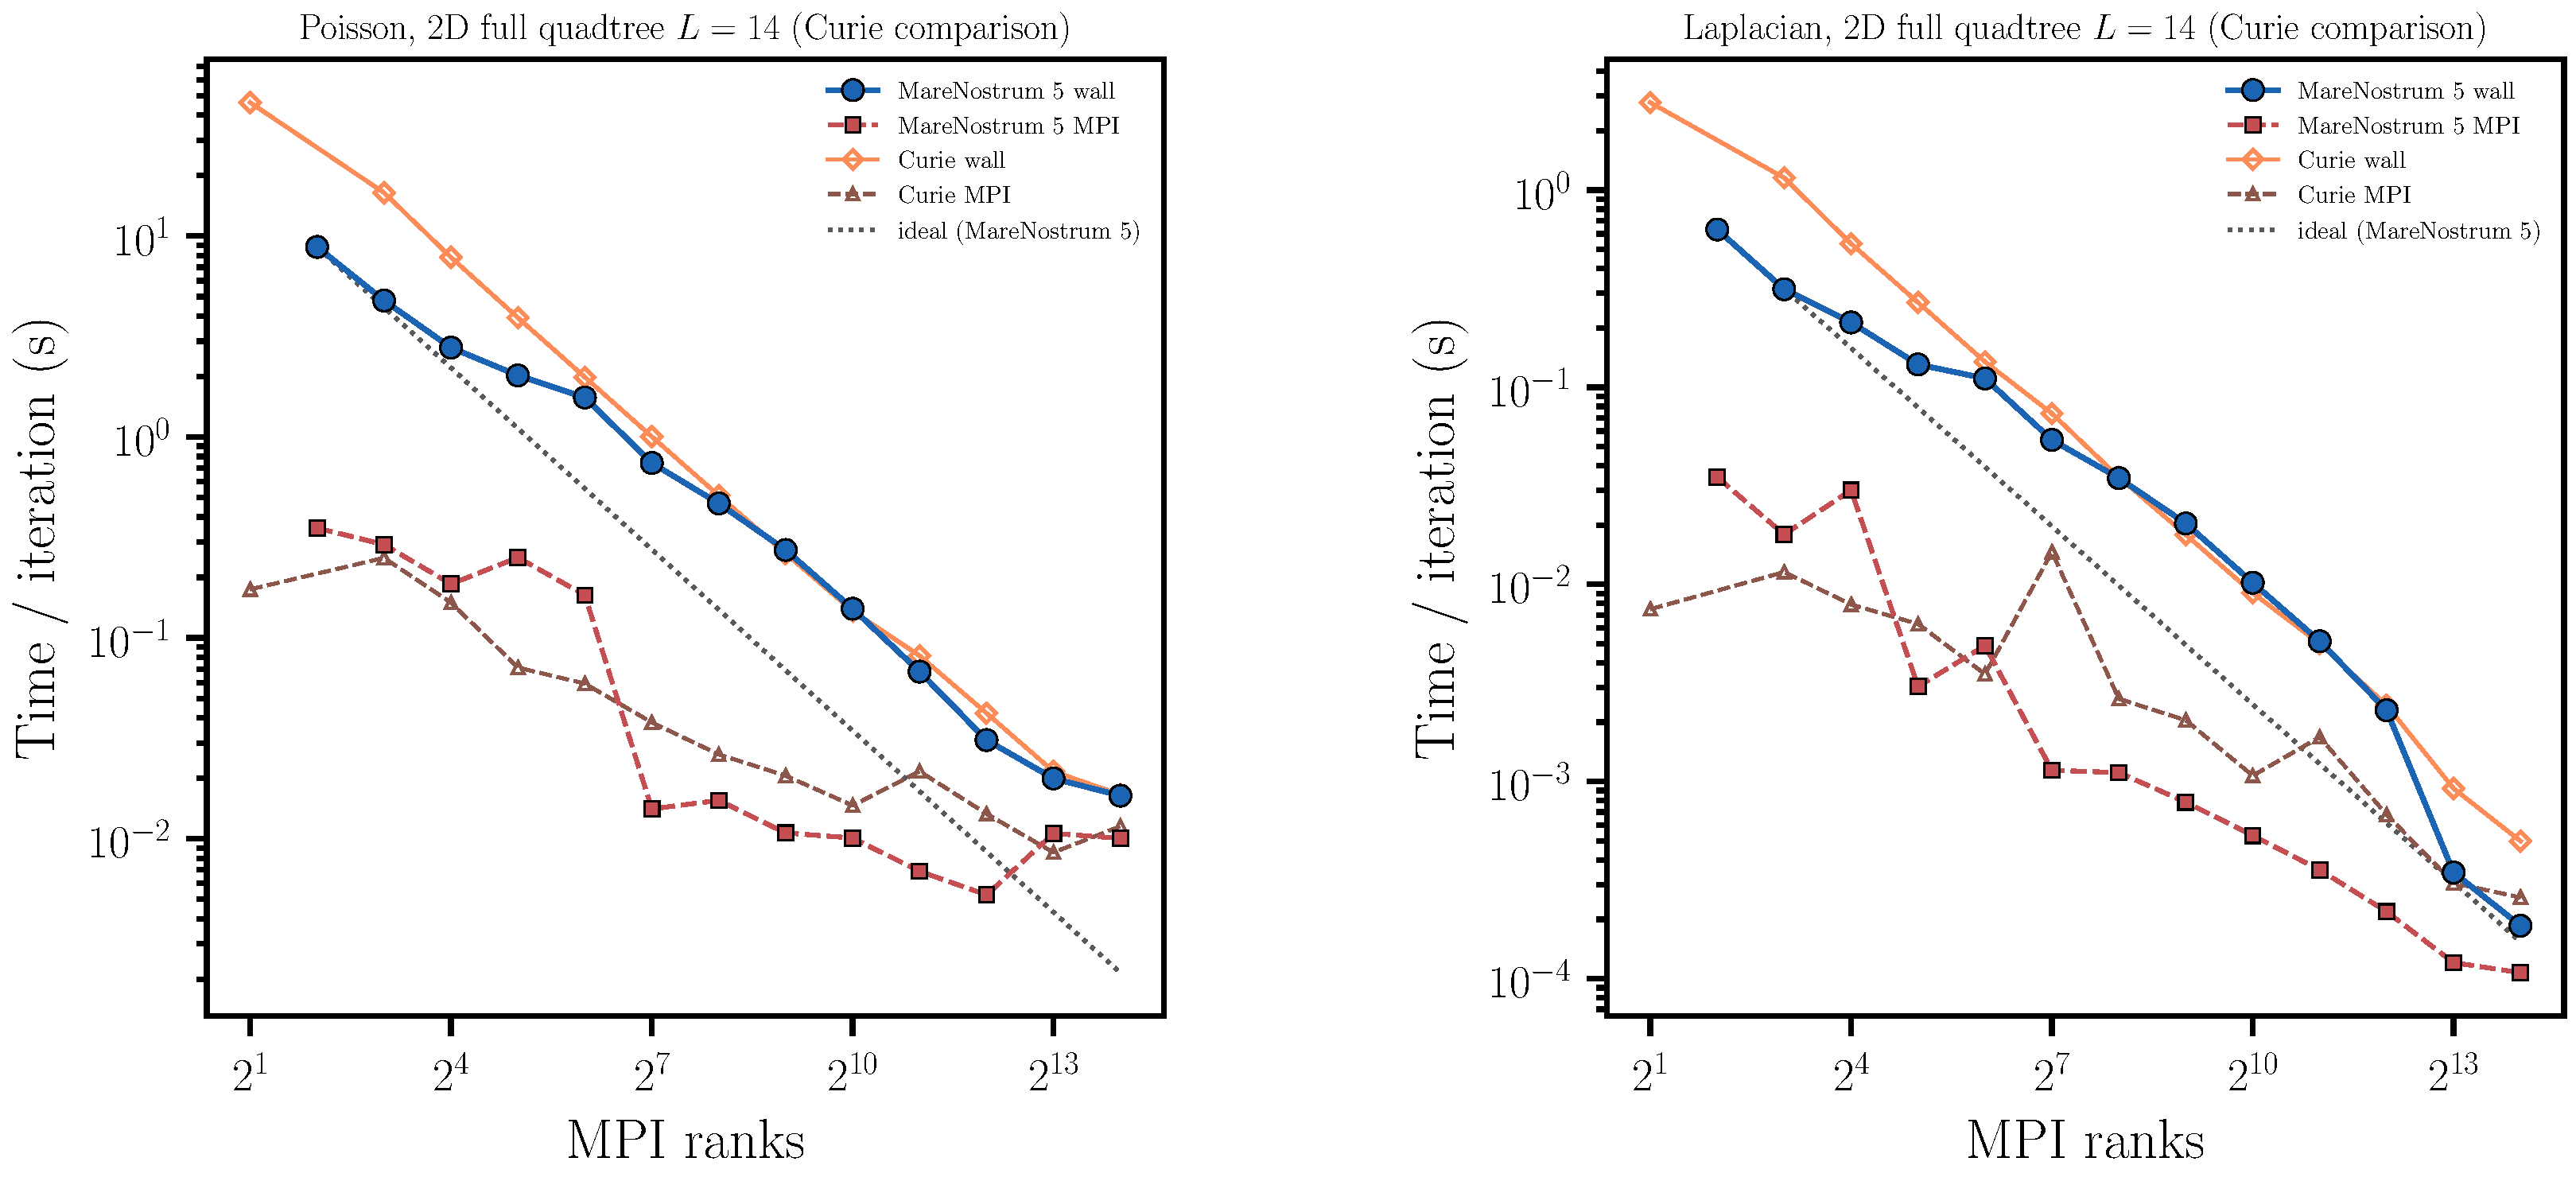
\includegraphics[width=\textwidth]{circle-L14.pdf}
  \caption{Strong scaling of the Poisson solve (left) and Laplacian operator
  (right) for the two-dimensional full-quadtree kernel at $L=14$. Solid curves
  show wall time per iteration and dashed curves show the measured MPI
  contribution. The grey dotted line is ideal scaling from the MareNostrum~5
  baseline. Curie data are the reference measurements distributed with the
  Basilisk test.}
  \label{fig:2d-kernel}
\end{figure}

The three-dimensional kernel uses a full octree at $L=9$, or $2^{27}$ cells.
On Snellius, the Poisson time falls from $19.34$~s at two ranks to
$0.0333$~s at 16,384 ranks. Most of the reduction has already been obtained
by 4,096 ranks, where the corresponding time is $0.0390$~s. Figure
\ref{fig:3d-kernel} therefore supplies both a broad scaling curve and a clear
diagnostic of the strong-scaling limit. The Occigen measurements provide an
independent reference for the same stock calculation.

\begin{figure}[htbp]
  \centering
  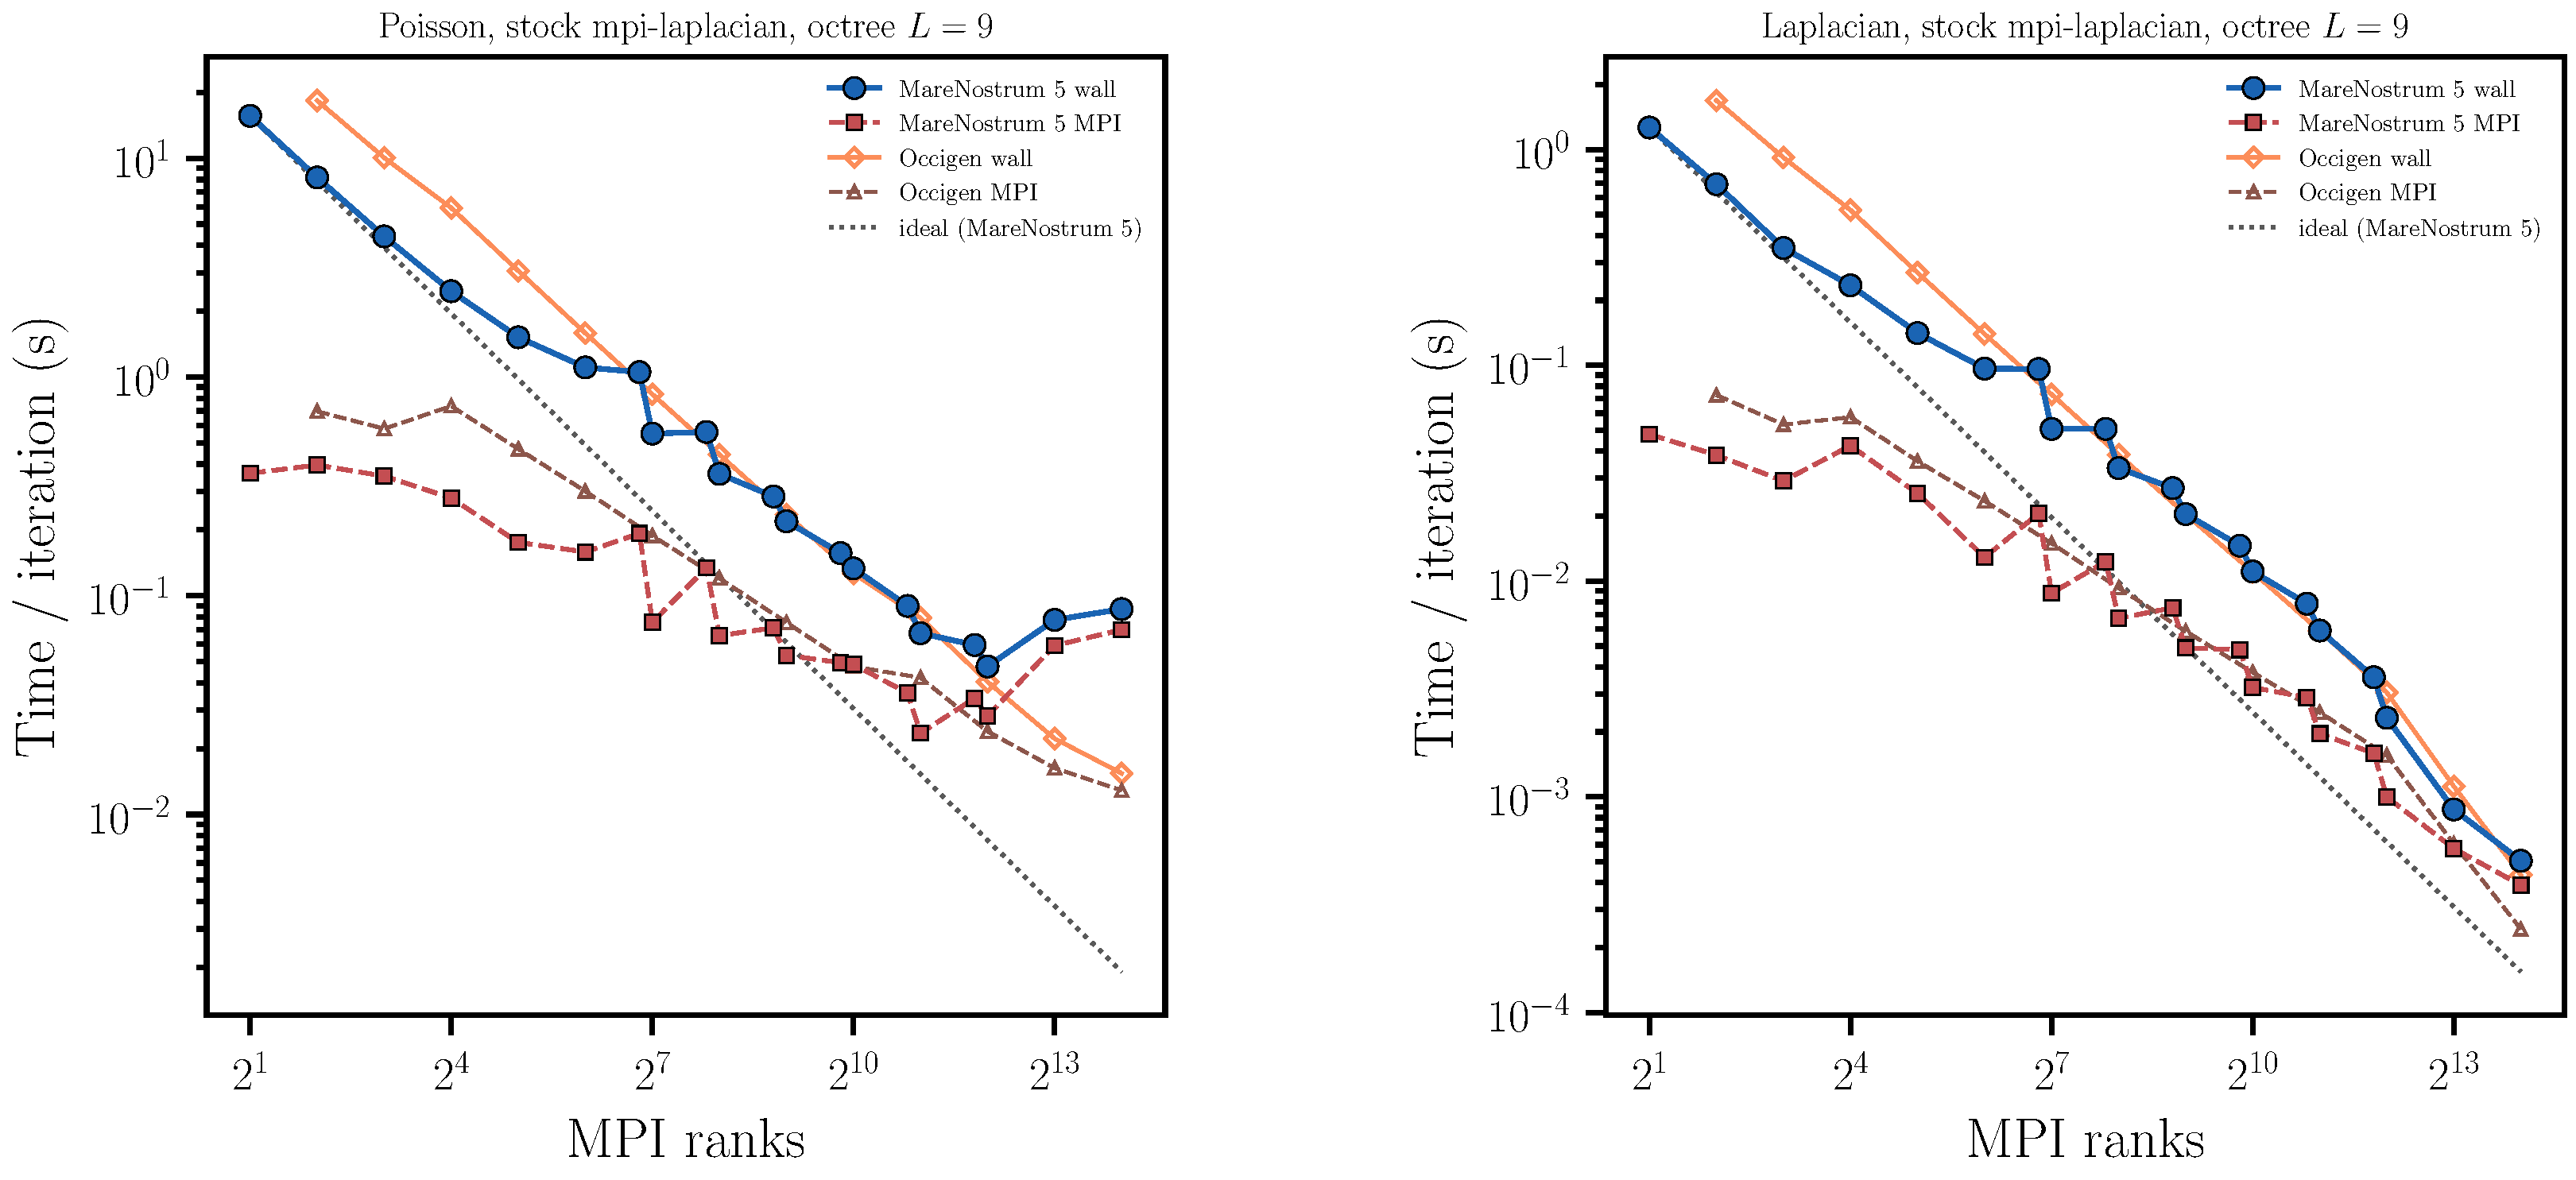
\includegraphics[width=\textwidth]{laplacian-L9.pdf}
  \caption{Strong scaling of the stock three-dimensional
  \texttt{mpi-laplacian} test on a full octree at $L=9$. Symbols and line
  styles follow Figure~\ref{fig:2d-kernel}; the reference machine is Occigen.
  The flattening of the Poisson curve beyond a few thousand ranks is the
  expected fixed-problem communication limit, not a loss of numerical
  correctness.}
  \label{fig:3d-kernel}
\end{figure}

These results show why one number is insufficient for procurement. A
low-rank timing measures core and memory performance, while the bend in the
curve measures the communication stack and the implementation of collective
operations. Both are relevant to production multiphase-flow calculations.

\section{Representative multiphase workload}

The application benchmark follows a drop driven by a surface-tension
gradient. The numerical formulation is the conservative, balanced treatment
of interfacial stresses described by Abu-Al-Saud, Popinet and
Tchelepi~\cite{abu-al-saud2018}. The cluster case adds timing, restart and
controlled output to the public Basilisk test without changing the physical
validation target.

Figure~\ref{fig:application-scaling} varies the amount of work in two ways.
Panel~(a) increases the spatial resolution of an axisymmetric uniform mesh.
Panel~(b) increases the number of drops in a planar domain while retaining
64 points per radius. The larger problems continue to benefit from additional
ranks after the smaller problems have saturated. This is the expected
application behaviour: the useful rank count grows with the work available
per rank. The present application dataset stops at 1,024 ranks, approximately
5.3 fully populated 192-core nodes, and should be used as small-scale evidence.

\begin{figure}[htbp]
  \centering
  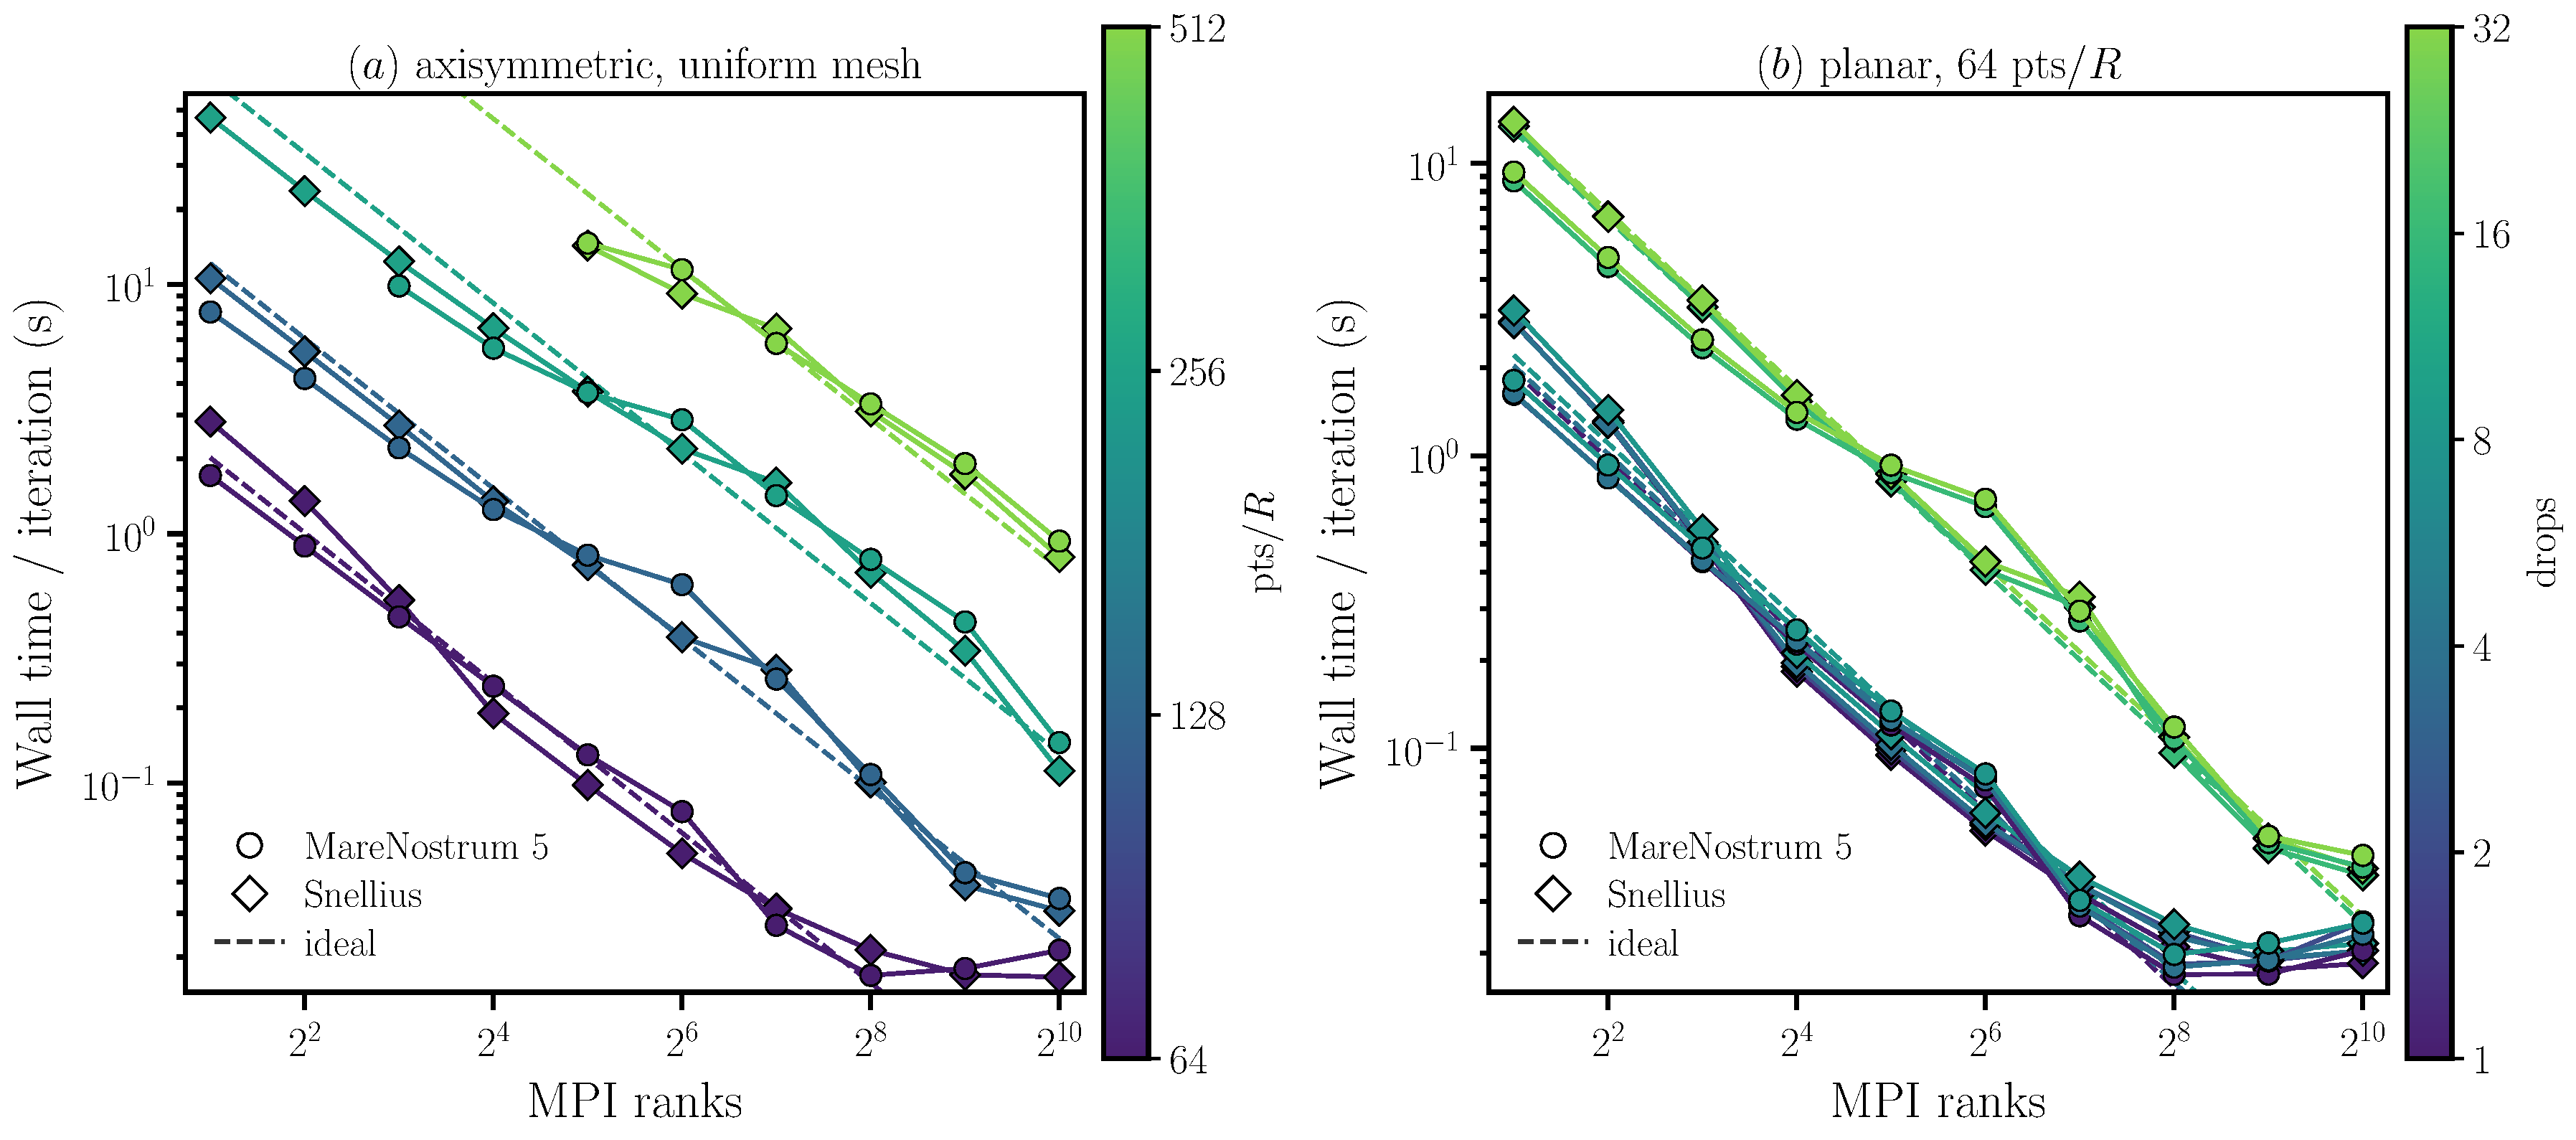
\includegraphics[width=\textwidth]{marangoni-uniform-ndrop-per-iter.pdf}
  \caption{Wall time per iteration for representative two-phase workloads on
  MareNostrum~5 and Snellius. (a) Axisymmetric uniform meshes, coloured by
  points per drop radius. (b) Planar uniform meshes at 64 points per radius,
  coloured by the number of drops. Dashed lines show ideal scaling for each
  workload. Each point is one recorded run; the current tables do not measure
  run-to-run variability.}
  \label{fig:application-scaling}
\end{figure}

The application remains useful only if it solves the intended flow. Figure
\ref{fig:validation} compares the computed drop speed with the analytical
terminal velocity and with the Basilisk reference data. The coarse-resolution
error follows the expected second-order trend through 32 points per radius;
the finer results approach the theoretical speed but should not be described
as a single second-order convergence range because their error plateaus.

\begin{figure}[htbp]
  \centering
  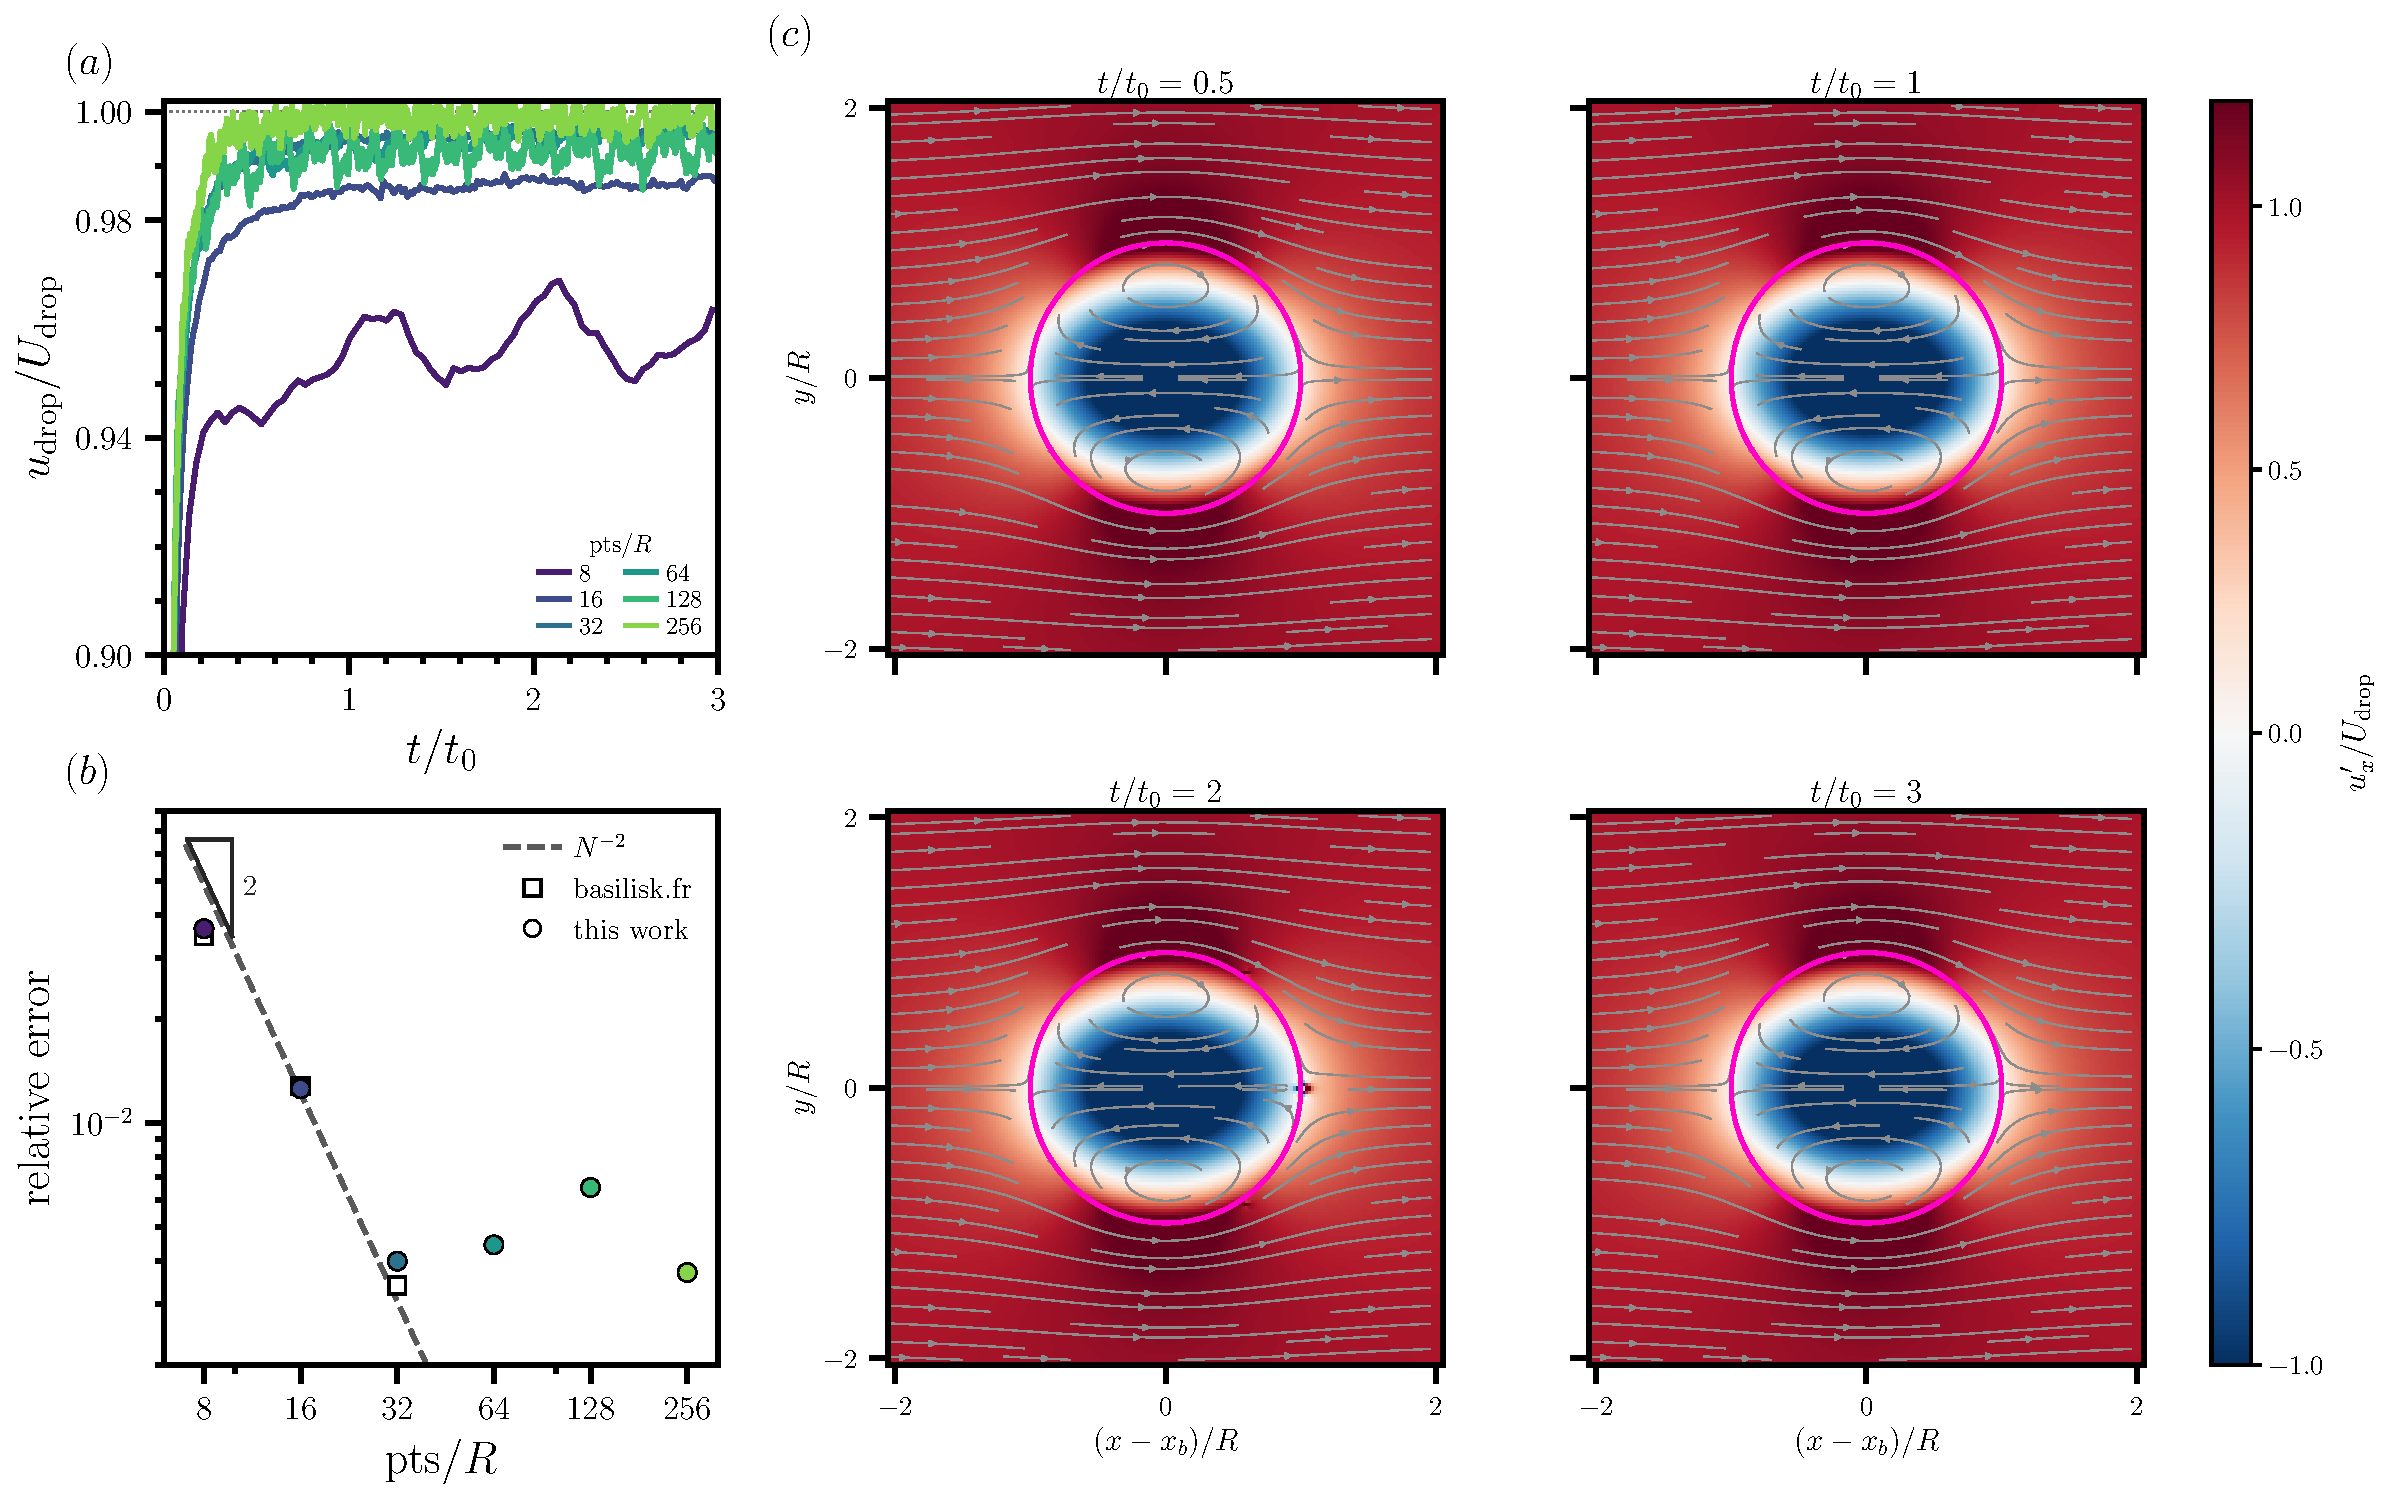
\includegraphics[width=\textwidth]{marangoni-validate-vt-fields.pdf}
  \caption{Numerical validation of the representative two-phase case.
  (a) Drop speed normalized by the theoretical terminal velocity.
  (b) Relative error with the $N^{-2}$ coarse-grid trend and the public
  Basilisk reference. (c) Resolved velocity fields at four times. The magenta
  curve marks the interface and the colour scale gives the streamwise
  velocity normalized by the terminal speed.}
  \label{fig:validation}
\end{figure}

\section{Qualification matrix for a 192-core node}

The present kernel measurements use powers of two in MPI rank count. They
reach 16,384 ranks on Snellius, equivalent to 85.3 fully populated 192-core
nodes. This brackets a 64-node test but does not demonstrate the requested
class above 100 nodes. Exact node-aligned rank counts must also be tested;
performance at 8,192 or 16,384 ranks should not be silently substituted for a
12,288-rank, 64-node measurement.

\begin{table}[htbp]
\centering
\small
\begin{tabularx}{\textwidth}{@{}lllX@{}}
\toprule
Class & Proposed nodes & MPI ranks & Present evidence \\
\midrule
Small & 1, 2, 4, 8, 10 & 192--1,920 & Kernel curves bracket the range; application to 1,024 ranks \\
Medium & 16, 32, 64 & 3,072--12,288 & Kernel data at 4,096 and 8,192 ranks; 64 nodes bracketed \\
Large & 128, 256 & 24,576--49,152 & Not yet measured; requires a scaled problem and memory pilot \\
\bottomrule
\end{tabularx}
\caption{Proposed node-aligned qualification points for a system with 192 CPU
cores per node. Existing evidence and proposed measurements are deliberately
separated.}
\label{tab:matrix}
\end{table}

For the small class, the current $L=9$ three-dimensional and $L=14$
two-dimensional problems can be retained as fixed-size strong-scaling tests.
For 16--64 nodes, a three-dimensional $L=10$ case should be added after a
memory check. The 128- and 256-node points require a larger problem, such as an
$L=11$ octree, after a short pilot has established memory use and initialization
cost. The purpose of the large case is to preserve enough cells per rank to
measure the network at scale rather than to time an already saturated problem.

The representative two-phase case should accompany the kernels at small and
medium scales. A large-scale application case should be promoted only after
its domain size, interface area and output policy have been fixed so that each
machine performs the same physical and numerical work.

\section{Reproducibility and reporting}

A procurement-quality result should record the following alongside every
timing:
\begin{itemize}
  \item the exact source revision and unmodified stock-test provenance;
  \item compiler, optimization flags, MPI implementation and launcher;
  \item node type, ranks per node, thread affinity and rank binding;
  \item mesh dimensionality, level, total cell count and cells per rank;
  \item wall time, MPI time, iteration count and any initialization excluded
        from the timed region; and
  \item at least three repeats after the initial qualification run, reporting
        the median and spread rather than only the best observation.
\end{itemize}

The current CSV files contain one observation for each configuration. They are
sufficient to locate scaling regimes and design the next campaign, but they do
not quantify system variability. Repeated node-aligned runs are therefore part
of the proposed qualification procedure.

\section{Conclusion}

Basilisk provides a compact CPU benchmark with a direct connection to
production multiphase-flow workloads. The stock Poisson and Laplacian kernels
separate local computation from MPI communication, while the verified
two-phase case tests interface reconstruction, surface tension and the full
projection step. Existing measurements cover the small class and bracket a
64-node, 192-core-per-node test. The next useful measurements are exact
node-aligned repeats and scaled three-dimensional problems at 128 and 256
nodes. This distinction keeps present evidence separate from the capabilities
that a future system must demonstrate.

\begin{thebibliography}{9}

\bibitem{basilisk-mpi-circle}
S.~Popinet,
\newblock \emph{Basilisk: MPI circle benchmark},
\newblock \url{https://basilisk.fr/src/test/mpi-circle.c}.

\bibitem{basilisk-mpi-laplacian}
S.~Popinet,
\newblock \emph{Basilisk: MPI Laplacian benchmark},
\newblock \url{https://basilisk.fr/src/test/mpi-laplacian.c}.

\bibitem{popinet2009}
S.~Popinet,
\newblock An accurate adaptive solver for surface-tension-driven interfacial
flows,
\newblock \emph{Journal of Computational Physics} \textbf{228} (2009),
5838--5866. \href{https://doi.org/10.1016/j.jcp.2009.04.042}{doi:10.1016/j.jcp.2009.04.042}.

\bibitem{abu-al-saud2018}
M.~O.~Abu-Al-Saud, S.~Popinet and H.~A.~Tchelepi,
\newblock A conservative and well-balanced surface tension model,
\newblock \emph{Journal of Computational Physics} \textbf{371} (2018),
896--913. \href{https://doi.org/10.1016/j.jcp.2018.02.022}{doi:10.1016/j.jcp.2018.02.022}.

\end{thebibliography}

\end{document}
